\chapter{Intra-vehicle Communications}
% Bus systems: basics
%   Protocols
%   K-Line
%   CAN
%   LIN
%   FlexRay
%   MOST
%   In-car Ethernet
% ECUs
% Safety

\section{Bus Systems}

% \subsection{ISO/OSU Layers: Router}
%
% \begin{figure}[!ht]
%   \centering
%   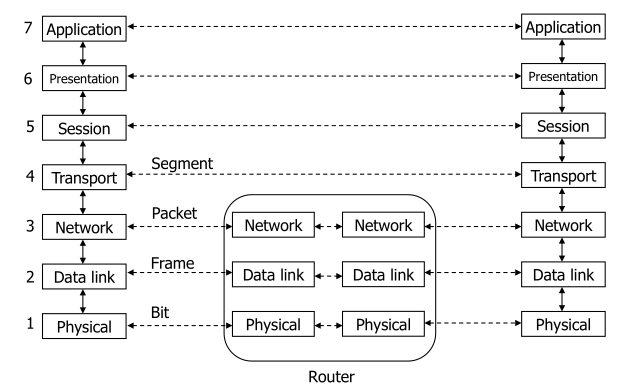
\includegraphics[width=0.4\textwidth]{./images/osi_router.png}
%   \caption{OSI Router}
%   \label{fig:osi_router}
% \end{figure}
%
% Da notare che se il router ha la parte di network separate, allora i due lati edllo strato network hanno protocolli diversi e il router deve fare da nterprete.
%
%
% \subsection{ISO/OSI Layers: Functions in Detail}
%
% \begin{itemize}
%   \item \textbf{Layer fisico}: trasmissione dei bit
%   \item \textbf{Layer data link}: trasmissione dei frame
%   \item \textbf{Layer network}: trasmette dei pacchetti
%   \item \textbf{Layer transport}: trasmissione sicura dei frammenti
%   \item \textbf{Layer session}: gestione della sessione
%   \item \textbf{Layer presentation}: definisce sintassi e semantica dell'informazione
%   \item \textbf{Layer application}: comunicazione fra applicazioni
% \end{itemize}



\subsection{Perchè usare i bus?}
Un bus che collega tutti i componenti al posto di avere una topologia a grafo completo ha i seguenti vantaggi:
\begin{itemize}
	\item \textbf{Riduzione dei costi}: meno cavi e meno connettori
	\item \textbf{Riduzione del peso}: meno cavi
	\item \textbf{Riduzione del volume}: meno cavi
	\item \textbf{Alta modularità}: modifica veicoli
	\item \textbf{Alta modularità}: cooperazione con OEM
	\item \textbf{Modularità}: riuso di moduli
	\item \textbf{Standardizzazione}: standardizzazione dei componenti e dei protocolli (meno errori scemi)
\end{itemize}




\subsection{Casi d'uso per intra-vehicle communications}

\begin{itemize}
	\item Driveline: Engine and transmission control
	\item Active Safety: Electronic Stability Programme (ESP)
	\item Passive Safety: Air bag, belt tensioners
	\item Comfort: Interior lighting, A/C automation
	\item Multimedia and Telematics: Navigation system, CD changer
\end{itemize}

La geolacaliuazione è fornita da protocolli di navigazione satellitare. I più famosi sono:
\begin{itemize}
	\item GPS: USA
	\item Galileo: EU
	\item Glonass: Russia
	\item Beidou: China
\end{itemize}

Altre soluzioni sono RTK(Real Time Kinematic)!!



\subsection{Classificazione: On-board-communcation}
\begin{itemize}
	\item Complex control and monitoring tasks: trasmissione dei dati tra ECUs(Engine Control Unit) e MMI(Man Machine Interface simile a HMI che sta per human machine interface)
	\item Simplification of wiring: rimpiazzare i fili di rame con bus per ridurre la complessità dei cablaggi
	\item Multimedia bus systems: Trasmette un sacco di dati per i sistemi di intrattenimento
\end{itemize}


\subsection{Classificazione: Off-board-communication(OBD connector)}
\begin{itemize}
	\item Diagnostics: diagnosi del veicolo
	\item Flashing: aggiornamento del software
	\item Debugging: debug del software
\end{itemize}

\subsection{Classificazione per casi d'uso e importanza}

\begin{table}[!ht]
	\begin{adjustbox}{width=\columnwidth,center}
		\begin{tabular}{|c|c|c|c|c|c|c|}
			\hline
			Application            & Message Length & Message rate & Data rate & Latency & Robustness & Cost \\
			\hline
			Control and monitoring &                & 2            & 2         & 3       & 3          & 2    \\
			\hline
			Simplified wiring      &                &              &           & 1       & 2          & 1    \\
			\hline
			Multimedia             & 1              & 2            & 3         & 1       & 1          & 3    \\
			\hline
			Diagnosis              &                &              &           &         &            & 1    \\
			\hline
			Flashing               & 2              &              & 2         &         & 1          &      \\
			\hline
			Debugging              &                & 1            & 1         & 2       &            &      \\
			\hline
		\end{tabular}
	\end{adjustbox}
	\caption{Classificazione per casi d'uso e importanza}
	\label{tab:classification_use_case}
\end{table}


\subsection{Classificazione SAE(Society of Automotive Engineers)}

\begin{table}
	\begin{adjustbox}{width=\columnwidth, center}
		\begin{tabular}{|c|c|c|c|}
			\hline
			Class & Data rate  & vantaggio                    & Dispositivi     \\
			\hline
			A     & $10kBit/s$ & Economico                    & Diagnosi        \\
			B     & $64kBit/s$ & Correzione errori            & Networking ECUs \\
			C     & $1MBit/s$  & Comunicazione in tempo reale & Drive train     \\
			D     & $10MBit/s$ & Bassa latenza                & X-By-Wire       \\
			\hline
		\end{tabular}
	\end{adjustbox}
	\caption{Classificazione SAE}
	\label{tab:classification_sae}
\end{table}



\subsection{Network Topologies}

\begin{itemize}
	\item \textbf{Repeter}: amplificazione del segnale a livello fisico
	\item \textbf{Bridge}: medium/timing adaptation, unfiltered forwarding a livello data link
	\item \textbf{Router}: medium/timing adaptation, filtered forwarding a livello network
	\item \textbf{Gateway}: medium/timing adaptation, filtered forwarding, protocol translation a livello application
\end{itemize}




ARRIVATO A PAGINA 20
